Sentiment and emotion analysis are two closely related yet distinct fields within natural language processing (NLP) and computational linguistics that aim to understand and interpret human affective states from textual data. The distinction between sentiment and emotion lies in their granularity and scope. While sentiment is broader typically focusing on identifying and categorizing the polarity of expressed opinions, such as positive, negative, or neutral sentiments, emotions are more intricate and multifaceted, reflecting the complexity of human psychological experiences. A foundational study by \citet{ekman1992there} identified six basic emotions—joy, anger, sadness, fear, surprise, and disgust—that are universally recognized across cultures. These emotions serve as a cornerstone for emotion analysis, providing a framework for understanding how affective states are expressed and perceived in text.
\newline

This chapter provides an overview of the existing research on sentiment and emotion analysis, covering approaches that leverage textual, visual, and multimodal data. Section~\ref{sec:text_analysis} focuses on text-based sentiment and emotion analysis, exploring classical machine learning and deep learning models used for this task. Section~\ref{sec:vision_analysis} shifts the focus to vision-based emotion analysis, discussing techniques for extracting emotions from images. Section~\ref{sec:multimodal_analysis} delves into multimodal sentiment and emotion analysis, outlining the models that integrate text and vision and the fusion strategies used to combine modalities effectively. Given the challenges of obtaining high-quality labeled data, Section~\ref{sec:weakly_supervised_back} discusses weakly supervised learning approaches in both text and vision domains. Finally, Section~\ref{sec:summary} summarizes key findings from the literature and highlights the gaps that motivate the research in this thesis.




\section{Text-Based Sentiment and Emotion Analysis}
\label{sec:text_analysis}

Text-based sentiment and emotion analysis has been a cornerstone of natural language processing (NLP) research for several decades, driven by the need to understand and quantify human emotions and opinions expressed in textual data. This field has evolved significantly, with methodologies ranging from simple lexicon-based approaches to sophisticated deep learning architectures. The ultimate goal of these techniques is to automatically classify the sentiment (positive, negative, or neutral) or emotion (e.g., joy, anger, sadness) conveyed in a given text, which has applications in areas such as customer feedback analysis, social media monitoring, and mental health assessment.

\subsection*{Lexicon-Based Methods}

One of the earliest and most straightforward approaches to sentiment and emotion analysis is the lexicon-based method. This technique relies on predefined dictionaries or lexicons, where each word is assigned a sentiment or emotion score. For example, the word \textit{happy} might be associated with a positive sentiment score, while \textit{sad} might carry a negative score. The overall sentiment or emotion of a sentence or document is then computed by aggregating the scores of the individual words, often using summation or weighted combination techniques. 
\newline
Popular resources for lexicon-based sentiment analysis include \textbf{SentiWordNet} \cite{baccianella-etal-2010-sentiwordnet}, which extends the WordNet lexical database by assigning sentiment scores to synsets (sets of synonyms), and domain-specific dictionaries tailored to particular industries or contexts. While these methods are computationally efficient and interpretable, they often require additional preprocessing steps to account for linguistic nuances such as \textbf{negation} (e.g., \textit{not happy}), \textbf{intensifiers} (e.g., \textit{very happy}), and \textbf{modifiers} (e.g., \textit{slightly happy}). These factors can significantly influence the final sentiment or emotion classification, making lexicon-based approaches somewhat limited in their ability to capture complex contextual information.

\subsection*{Classical Machine Learning Approaches}

With the advent of machine learning, researchers began to explore more data-driven methods for sentiment and emotion analysis. Classical machine learning algorithms such as \textbf{Na\"ive Bayes}, \textbf{Support Vector Machines (SVMs)}, and \textbf{Logistic Regression} became popular choices for this task. These models are typically trained on labelled datasets, where each text sample is annotated with its corresponding sentiment or emotion label. 
\newline
A critical aspect of these approaches is \textbf{feature engineering}, where handcrafted features are extracted from the text to represent it in a way that is suitable for machine learning. Common features include \textbf{word n-grams} (sequences of \textit{n} words), \textbf{part-of-speech (POS) tags}, and \textbf{syntactic or semantic cues} such as dependency relations or sentiment-bearing phrases. The performance of these models heavily depends on the quality and relevance of the engineered features, as they do not inherently learn contextual representations of words. Despite their limitations, these methods laid the groundwork for more advanced techniques by demonstrating the potential of data-driven approaches in NLP.

\subsection*{Deep Learning and Neural Networks}

The introduction of \textbf{deep learning} marked a significant shift in sentiment and emotion analysis, moving away from manual feature engineering toward \textbf{automatically learned representations} of text. Early deep learning architectures for this task often employed \textbf{Recurrent Neural Networks (RNNs)} \cite{Mikolov:2010wx}, which are designed to process sequential data by maintaining a hidden state that captures information from previous time steps. Variants such as \textbf{Long Short-Term Memory (LSTM)} networks \cite{10.1162/neco.1997.9.8.1735} and \textbf{Gated Recurrent Units (GRUs)} \cite{cho2014learningphraserepresentationsusing} addressed the \textbf{vanishing and exploding gradient problems} commonly encountered in standard RNNs. These architectures are particularly effective for sentiment and emotion analysis because they can model long-range dependencies in text, capturing the influence of earlier words on the sentiment or emotion expressed later in a sentence.
\newline

\textbf{Bidirectional RNNs} further enhanced this capability by processing text in both forward and backward directions, allowing the model to incorporate context from both preceding and succeeding words \cite{1556215}. This bidirectional approach proved especially useful for tasks requiring a comprehensive understanding of sentence structure and meaning.

\subsection*{Convolutional Neural Networks (CNNs) for Text}

In parallel with RNNs, \textbf{Convolutional Neural Networks (CNNs)} were also adapted for text-based sentiment and emotion analysis \cite{10.5555/2999134.2999257}. Originally designed for image processing, CNNs were repurposed for NLP tasks by applying one-dimensional filters to \textbf{word embeddings} (dense vector representations of words). These filters extract local n-gram features, capturing patterns and relationships within small windows of text. The most salient features are then aggregated through \textbf{pooling layers} before being passed to a classification layer.
\newline

While CNNs have demonstrated strong performance in certain NLP tasks, they are less effective at modeling \textbf{long-range dependencies} in text. This limitation arises because CNNs are designed to capture local spatial relationships, making them less suitable for tasks that require a global understanding of context or relationships between distant parts of a sentence. As a result, CNNs have gradually been overshadowed by more advanced architectures that better address these challenges.

\subsection*{Attention Mechanisms and Transformers}

A major breakthrough in sentiment and emotion analysis came with the introduction of \textbf{attention mechanisms} \cite{Bahdanau2014NeuralMT}, which enable models to selectively focus on the most relevant parts of a sentence rather than processing it sequentially. Attention-based architectures improved the interpretability of results by highlighting which words or phrases contributed most to the predicted sentiment or emotion. This innovation paved the way for \textbf{Transformers} \cite{vaswani2023attentionneed}, which revolutionized NLP by eliminating the need for recurrent processing altogether.
\newline

Transformers rely on a \textbf{self-attention mechanism} that allows the model to attend to different positions in a sequence, enabling it to learn \textbf{contextualized embeddings} efficiently. This architecture has become the foundation for many state-of-the-art models in NLP, including \textbf{BERT} \cite{DBLP:journals/corr/abs-1810-04805} and \textbf{GPT} \cite{Radford2018ImprovingLU}. These \textbf{pretrained language models} leverage vast amounts of unlabelled text to learn general-purpose representations of language, which can then be fine-tuned for specific tasks such as sentiment or emotion classification.

\subsection*{Pretrained Language Models and Fine-Tuning}

Pretrained models like BERT and GPT have dominated the field of sentiment and emotion analysis due to their ability to capture rich contextual information. These models are typically fine-tuned on task-specific datasets by appending a classification layer on top of their final hidden representations. \textbf{RoBERTa}, introduced in the paper titled \emph{RoBERTa: A Robustly Optimized BERT Pretraining Approach} by \cite{DBLP:journals/corr/abs-1907-11692}, improves upon BERT by optimizing several key aspects of the pretraining process. It trains longer with larger batches and more data, addressing BERT's undertraining. The next sentence prediction (NSP) objective is removed, as it was found unnecessary, and dynamic masking is introduced, generating new masks for each sequence instead of using static ones. RoBERTa also trains on longer sequences to capture broader dependencies and uses a larger, more diverse dataset. These changes collectively enhance performance, enabling RoBERTa to achieve state-of-the-art results on several benchmarks. 
\newline

\cite{nguyen-etal-2020-bertweet} introduce BERTweet, the first large-scale pre-trained language model specifically designed for English Tweets, using the same architecture as BERT-base and trained on an 80GB corpus of 850 million Tweets following the RoBERTa pre-training procedure. BERTweet outperforms strong baselines like RoBERTa-base and XLM-R-base on three downstream Tweet NLP tasks—Part-of-speech tagging, Named-entity recognition, and text classification (sentiment analysis and irony detection)—achieving new state-of-the-art results, particularly in novel and emerging entity recognition and text classification. 
\newline

Moreover variants such as \textbf{DistilBERT} \cite{sanh2020distilbertdistilledversionbert} and \textbf{T5} \cite{raffel2023exploringlimitstransferlearning} have further optimized these architectures by modifying training objectives and data settings, resulting in more efficient and effective models. The widespread adoption of transformer-based models has led to significant improvements in performance across diverse datasets and languages. However, challenges remain, particularly in capturing domain-specific nuances and handling multimodal data (e.g., combining text with images or audio). Ongoing research continues to explore advanced techniques such as \textbf{domain adaptation}, \textbf{transfer learning}, and \textbf{multimodal sentiment analysis} to address these limitations and further enhance the capabilities of text-based sentiment and emotion analysis systems.

\section{Vision-Based Sentiment and Emotion Analysis}
\label{sec:vision_analysis}

While text-based methods have historically dominated the field of sentiment and emotion analysis, vision-based approaches have emerged as a powerful alternative, particularly in applications where facial expressions, body language, and other visual cues are central to understanding emotional states. Vision-based sentiment analysis leverages images or video data to infer the emotional states of individuals, offering a complementary perspective to text-based methods. This approach is especially valuable in scenarios where textual data is sparse, ambiguous, or unavailable, such as in video surveillance, or human-computer interaction.
\newline

The ability to analyze visual data for sentiment and emotion has broad implications across multiple domains, including psychology, marketing, healthcare, and entertainment. For instance, in healthcare, vision-based emotion analysis can be used to monitor patients' emotional well-being \cite{6940284}. Despite its potential, vision-based sentiment analysis presents unique challenges, such as the need to account for variations in lighting, pose, occlusion, and cultural differences in emotional expression \cite{10.1145/3240508.3240574}.

\subsection*{Traditional Feature Extraction}

Early approaches to vision-based sentiment analysis relied heavily on handcrafted feature extraction techniques, which aimed to capture low-level visual patterns indicative of emotional states. Two of the most widely used methods were the Scale-Invariant Feature Transform (SIFT) \cite{Lowe2004DistinctiveIF} and the Histogram of Oriented Gradients (HOG) \cite{1467360}. These techniques extract features such as edges, corners, and gradients from images, which are then used as input to classical machine learning models like SVMs or KNNs.
\newline

While these methods are computationally efficient and interpretable, they have significant limitations. Handcrafted features often fail to capture high-level semantic information, such as the context or subtle nuances of emotional expressions \cite{6940284}. For instance, they may struggle to distinguish between a genuine smile and a forced one or to recognize complex emotions like confusion or ambivalence.

\subsection*{Convolutional Neural Networks (CNNs)}

The advent of Convolutional Neural Networks (CNNs) marked a paradigm shift in vision-based sentiment analysis \cite{lecun_deep_2015}. Unlike traditional methods, which rely on handcrafted features, CNNs automatically learn hierarchical representations of visual data through multiple layers of convolutional filters. This capability allows CNNs to capture both low-level features (e.g., edges and textures) and high-level semantic information (e.g., facial expressions and emotional context).
\newline

The breakthrough moment for CNNs in computer vision came with the introduction of \textbf{AlexNet} in 2012 \cite{10.5555/2999134.2999257}, which demonstrated the power of deep convolutional layers in learning discriminative features from images. AlexNet's success was followed by a series of increasingly sophisticated architectures, such as \textbf{VGGNet} \cite{simonyan2015deepconvolutionalnetworkslargescale}, \textbf{Inception} (\cite{szegedy2015rethinkinginceptionarchitecturecomputer}, and \textbf{ResNet} \cite{he2015deepresiduallearningimage}. ResNet, in particular, introduced residual connections to address the vanishing gradient problem, enabling the training of very deep networks with hundreds of layers. These advancements significantly improved the ability of CNNs to recognize emotions from facial expressions and other visual cues, achieving state-of-the-art performance on benchmark datasets.
\newline

One of the key advantages of CNNs is their ability to leverage pretrained models, such as those trained on large-scale datasets like ImageNet \cite{5206848}. By fine-tuning these models for sentiment analysis tasks, researchers can achieve high accuracy and generalization even with relatively small amounts of labeled data \cite{yosinski2014transferablefeaturesdeepneural}. For example, a CNN pretrained on ImageNet can be adapted to recognize facial expressions by retraining its final layers on a dataset of annotated facial images. This transfer learning approach has become a standard practice in vision-based sentiment analysis, significantly reducing the need for large annotated datasets.
\newline

Recent studies have explored modifications to CNN architectures to improve their performance in emotion recognition. For instance, \citet{limami_contextual_2024} advance contextual emotion detection in images by proposing two deep learning models—a Deep Convolutional Neural Network (DCNN) and a VGG19-based model—that integrate 26 discrete emotion categories with three continuous emotional dimensions (valence, arousal, dominance) to improve emotion recognition accuracy. By combining body features and contextual features, the models achieved a mean Average Precision (mAP) of 78.39\% and 79.60\%, respectively, outperforming previous methods and demonstrating the importance of context in interpreting emotions.
\newline

\citet{al-halah2020} introduce SmileyNet, a novel approach for visual sentiment analysis that leverages emoji-based image embeddings to address the limitations of small-scale sentiment datasets. By constructing a large-scale dataset of 4 million images from Twitter, annotated with associated emojis, the authors train a deep neural network to predict emojis, creating a compact and sentiment-aligned embedding. This embedding outperforms traditional object-based representations (e.g., ImageNet) in visual sentiment analysis and fine-grained emotion classification, achieving state-of-the-art results on benchmark datasets. Additionally, hybrid models combining Multi-Scale Dynamic 1D CNN and Gated Transformer have shown high accuracy in EEG-based emotion recognition, highlighting the effectiveness of combining spatial-spectral features with global dependencies \cite{cheng_eeg-based_2024}
\newline

Despite their success, CNNs are not without limitations. They require substantial computational resources for training and inference, particularly for deep architectures like ResNet \cite{he2015deepresiduallearningimage}. Additionally, CNNs are primarily designed to process local spatial information, which can make it challenging to capture global relationships within an image. This limitation has spurred the development of alternative approaches, such as Vision Transformers (ViTs), which aim to address these shortcomings.

\subsection*{Vision Transformers (ViTs)}

The latest advancements in vision-based sentiment analysis have been driven by \textbf{Vision Transformers (ViTs)} \cite{dosovitskiy2021imageworth16x16words} and their variants, such as \textbf{Swin Transformers} \cite{liu2021swintransformerhierarchicalvision}. Unlike CNNs, which process images through convolutional filters, ViTs treat images as sequences of patches and apply self-attention mechanisms to capture global relationships within the visual data. This approach enables a more comprehensive understanding of complex emotional expressions, particularly in scenarios where subtle cues are critical.
\newline

ViTs were initially inspired by the success of transformers in natural language processing (NLP), where self-attention mechanisms have proven highly effective at modeling long-range dependencies in text \cite{vaswani2023attentionneed}. By adapting this architecture to visual data, ViTs can capture both local and global features, making them particularly well-suited for tasks like emotion recognition, where context and fine-grained details are important \cite{dosovitskiy2021imageworth16x16words}. For example, a ViT can analyze the relationship between different facial regions (e.g., eyes, mouth, and eyebrows) to infer emotions like surprise or disgust.
\newline

One of the most notable variants of ViTs is the Swin Transformer, which introduces a hierarchical feature extraction process. Swin Transformers divide an image into non-overlapping windows and apply self-attention within each window, reducing computational complexity while maintaining the ability to capture global relationships. This hybrid approach combines the strengths of ViTs and traditional CNNs, enabling state-of-the-art performance on various benchmarks. 
\newline

ViTs have also paved way for multi-modal approaches such as \textbf{CLIP (Contrastive Language-Image Pretraining)} \cite{radford2021learningtransferablevisualmodels} have shown remarkable potential in tasks that involve vision and language integration. This capability is particularly relevant for emotion recognition tasks that rely on both visual cues and associated text, such as social media posts containing images and captions.
\newline

The success of ViTs and their variants, along with multi-modal models like CLIP, has opened up new possibilities for vision-based sentiment analysis. These models are particularly effective at handling complex scenarios, such as group emotion recognition or the analysis of subtle micro-expressions \cite{liu2021swintransformerhierarchicalvision}. \citet{soni_vision_2024} apply a ViT-based model was applied to the FER-2013 dataset for emotion detection in human-computer interaction (HCI). The study emphasized meticulous preprocessing, data augmentation, and fine-tuning of the ViT model, achieving a testing accuracy of 70\%. However, they also come with challenges, including high computational costs and the need for large amounts of training data. Future research is likely to focus on improving the efficiency and scalability of these models, as well as exploring their application in real-world settings.


\section{Multimodal Sentiment and Emotion Analysis}
\label{sec:multimodal_analysis}

Multimodal sentiment/emotion analysis is a rapidly evolving field focused on understanding human emotions by integrating data from multiple modalities, such as text, audio, and visual inputs. Because human communication naturally spans these different modalities, relying on a single source of information often results in incomplete or inaccurate emotion recognition. As a result, multimodal approaches are increasingly critical for achieving more robust and comprehensive emotion analysis.

\subsection{Multimodal Models}

Several multimodal models have been developed to address the complexities of sentiment and emotion analysis. This section highlights three notable examples: VisualBERT, MuAL, and CLIP.

\paragraph{VisualBERT.}
VisualBERT \cite{li2019visualbertsimpleperformantbaseline} is a multimodal transformer model designed for vision-language tasks. It unifies visual and textual inputs within the same architecture, leveraging BERT's bidirectional attention mechanism to jointly process image regions and text tokens. VisualBERT has shown strong performance in tasks such as visual question answering and image captioning. However, it requires aligned image-text pairs during training, which can constrain its flexibility in handling unaligned multimodal data.

\paragraph{MuAL (Multimodal Sentiment Analysis with Cross-Modal Attention and Difference Loss).}
MuAL \cite{deng_mual_2024} is a recent approach that integrates cross-modal attention and a difference loss to enhance model robustness in multimodal sentiment analysis. By minimizing the gap between image and text representations, MuAL improves performance over traditional unimodal methods and demonstrates strong transfer learning capabilities. Notably, it outperforms baseline models even when its pre-trained parameters are frozen, making it particularly suitable for real-world applications where computational efficiency and generalization are crucial.

\paragraph{Multi-Level Semantic Reasoning Network (MULSER) for fine-grained multimodal emotion classification.} This paper introduced by \citet{9920172} addresses the limitation of traditional sentiment polarity analysis (e.g., positive/negative) by distinguishing nuanced emotions (e.g., happiness vs. love). MULSER leverages graph attention networks to model semantic relationships at multiple levels: for images, it constructs object-level, global-level, and joint regional-global graphs to capture interactions between local objects and contextual concepts; for text, it builds word-level graphs to enhance interdependencies between words. A cross-modal attention fusion module integrates the enriched visual and textual features, enabling complementary reasoning. Experiments demonstrate MULSER's superiority over state-of-the-art methods, achieving significant improvements in accuracy and F1 score. Ablation studies confirm the effectiveness of each component, emphasizing the importance of semantic reasoning and cross-modal interaction.


\subsubsection*{CLIP}
CLIP (Contrastive Language–Image Pre-training) is a neural network model that aligns textual and visual modalities within a shared embedding space. This alignment enables various multimodal tasks without the need for task-specific labeled datasets. Departing from traditional supervised learning approaches that rely on domain-specific annotations, CLIP employs a zero-shot learning paradigm, allowing it to generalize across tasks by capturing the relationships between text and images without explicit fine-tuning \cite{radford2021learningtransferablevisualmodels}.
\newline

CLIP is trained using a contrastive learning objective that maximizes the cosine similarity for matched image-text pairs while minimizing it for mismatched pairs. By doing so, CLIP learns representations that effectively capture semantic relationships across modalities. This capability allows the model to perform tasks such as image classification by comparing embedded textual labels (e.g., “a photo of a dog”) with image embeddings in a shared latent space. Figure \ref{fig:sidebyside} illustrates the contrastive learning framework employed in CLIP.
\newline

\begin{figure}[h]
\centering
\begin{minipage}[b]{0.45\textwidth}
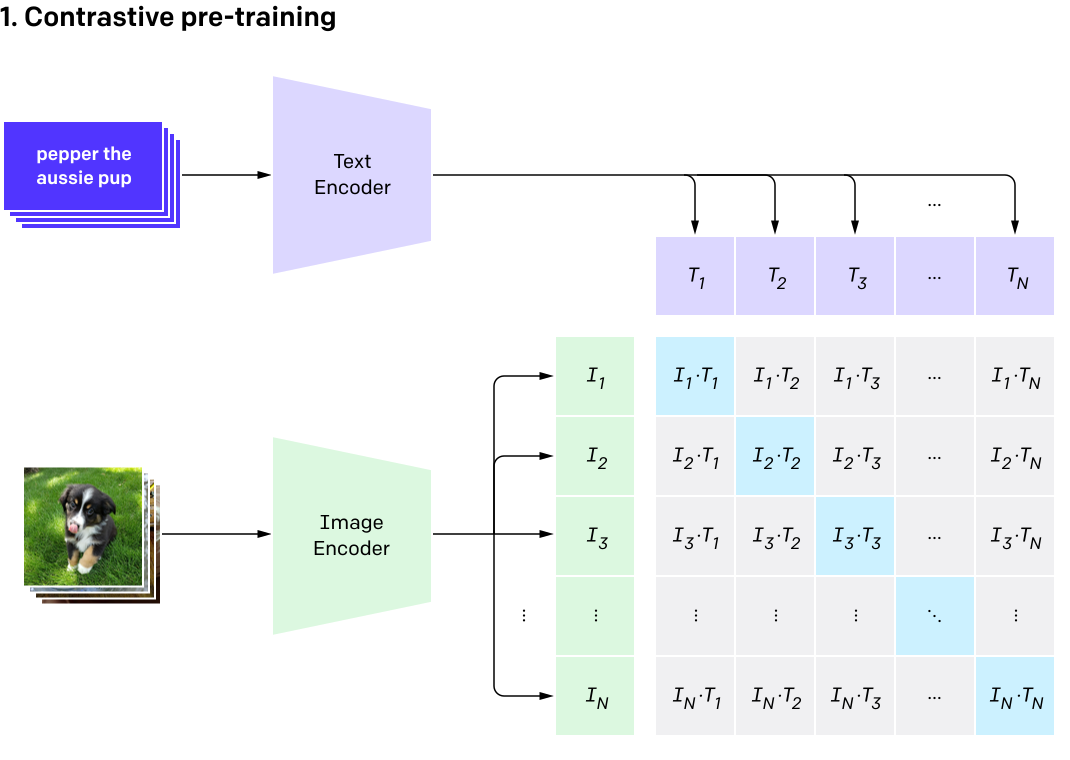
\includegraphics[width=\textwidth]{images/overview-a-clip.png}
\caption{Contrastive Pre-training}
\label{fig:contrastive_loss }
\end{minipage}
\hfill
\begin{minipage}[b]{0.45\textwidth}
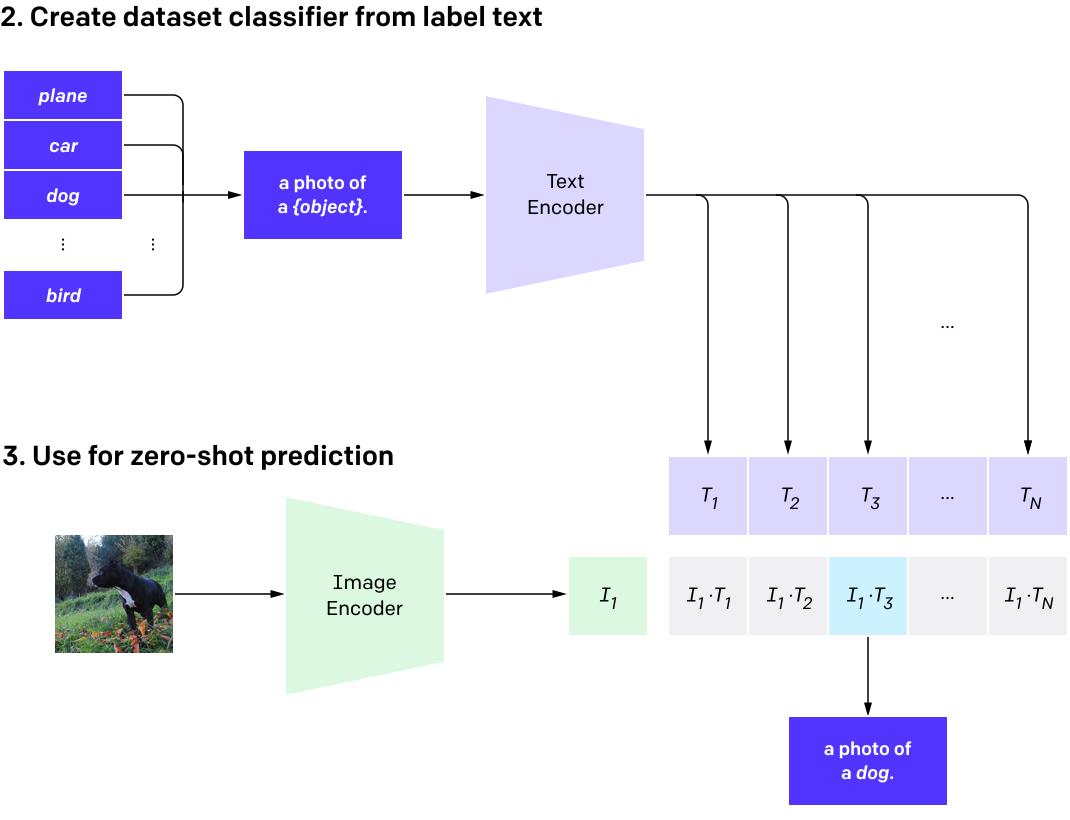
\includegraphics[width=\textwidth]{images/overview-b-clip.png}
\caption{Creation of dataset classifier and final prediction}
\label{fig:clip_zero }
\end{minipage}
\caption{Approach to training CLIP and Inference \cite{radford2021learningtransferablevisualmodels}}
\label{fig:sidebyside}
\end{figure}

CLIP was trained on approximately 400 million image-text pairs collected from the internet, leveraging the natural co-occurrence of images and their descriptions instead of manual annotations. This large and diverse dataset allows the model to learn broad visual-textual relationships, making it applicable to a variety of tasks. CLIP’s architecture consists of two main components: an image encoder (commonly a Vision Transformer \cite{dosovitskiy2021imageworth16x16words}) and a text encoder (based on transformer architectures like GPT or BERT \cite{Radford2018ImprovingLU, DBLP:journals/corr/abs-1810-04805}). Both encoders produce high-dimensional embeddings that are projected into a shared latent space, where contrastive learning aligns matched image-text pairs and separates mismatched ones.
\newline

To further improve generalization, CLIP leverages data augmentation techniques—such as resizing, cropping, and color adjustments—and large batch sizes that provide a diverse set of negative examples during contrastive learning. One of CLIP’s most significant strengths is its zero-shot learning paradigm, which allows the model to interpret natural language as a “programming interface.” In this setup, text prompts are embedded into the shared latent space and compared to image embeddings. Tasks like image classification, object detection, and text-based image retrieval can thus be performed without any task-specific fine-tuning (Figure \ref{fig:clip_zero }).
\newline

CLIP’s foundational principles have informed other multimodal models, such as LXMERT \cite{tan2019lxmertlearningcrossmodalityencoder}, which employs cross-attention mechanisms for visual question answering and image captioning. These advances extend CLIP’s core ideas to a variety of multimodal applications, including affective computing and social media analysis.



\subsection{Fusion strategies}

Multimodal data fusion has emerged as a critical area of research in machine learning, driven by the increasing availability of diverse data sources such as text, images, audio, and video. The integration of these modalities offers opportunities to enhance model performance by leveraging complementary information. However, the challenges of aligning and fusing heterogeneous data types necessitate sophisticated techniques. This sub-section summarizes insights from two key papers: \emph{Effective Techniques for Multimodal Data Fusion: A Comparative Analysis} by \cite{pawlowski_effective_2023} and \emph{Multimodal Alignment and Fusion: A Survey} by \cite{li_multimodal_2024}. These works provide a comprehensive overview of fusion techniques, their applications, and the challenges associated with multimodal integration.

\subsubsection{Fusion Techniques and Their Applications}

Pawlowski et al. focus on three primary fusion techniques—\textbf{late fusion}, \textbf{early fusion}, and \textbf{sketch representation}—and evaluate their effectiveness in classification tasks. Their findings highlight the dominance of \textbf{late fusion} in scenarios where one modality is dominant or unimodal models already perform well. For instance, in the Amazon Reviews dataset, late fusion achieved the highest accuracy (0.969) by combining textual and visual modalities. This technique processes each modality independently and combines their outputs at the decision level, making it robust to modality-specific noise and variability.
\newline

In contrast, \textbf{early fusion} integrates modalities at the input level by concatenating their embeddings. While this approach is beneficial when modalities are interdependent, it often underperforms compared to late fusion, as seen in the MovieLens datasets. Early fusion's reliance on combined embeddings can lead to information loss or redundancy, particularly when modalities are not equally informative.
\newline

The \textbf{sketch representation} technique, which transforms modalities into a common space using hash functions, offers a memory-efficient alternative. Although it underperformed in classification tasks, its scalability and computational efficiency make it suitable for large-scale applications like recommendation systems. Pawłowski et al. emphasize that the choice of fusion technique should be guided by task requirements, modality impact, and memory constraints.
\newline

Li and Tang provide a comprehensive overview of multimodal fusion techniques by categorizing them into four main types: encoder-decoder fusion, kernel-based fusion, graphical fusion, and attention-based fusion. Each of these methods addresses the challenge of integrating information from different modalities, such as text, images, and audio, to improve performance in various machine learning tasks.
\newline

\textbf{Encoder-Decoder Fusion:} This approach involves using separate encoders to process different modalities and then combining their outputs through a decoder. The encoders transform raw input data (e.g., images, text) into a shared latent space, where the decoder generates a unified representation. This method is particularly useful in tasks like image captioning and video summarization, where the goal is to generate a coherent output from multiple input modalities \citet{8269806}.
\newline


Attention-Based Fusion: Attention mechanisms have gained significant attention in recent years due to their ability to dynamically weight the importance of features across modalities. Li and Tang emphasize the role of attention mechanisms in capturing long-range dependencies and inter-modal interactions. Advanced models like ALBEF (Align before Fuse) and BLIP (Bootstrapped Language-Image Pretraining) further refine this approach by aligning modalities before fusion and leveraging large-scale pretraining to improve performance \cite{li2021alignfusevisionlanguage, li2022blipbootstrappinglanguageimagepretraining}.
\newline

These attention-based methods excel in tasks like social media analysis and emotion recognition, where understanding the nuanced interactions between text, images, and other modalities is crucial. For example, in social media analysis, attention mechanisms can help identify the most relevant posts or images that contribute to a trending topic, while in emotion recognition, they can dynamically weight the importance of facial expressions, voice tone, and textual content to accurately infer emotional states \cite{poria_review_2017}.

\subsubsection{Alignment Challenges and Conclusion}
A critical aspect of multimodal fusion is alignment, which ensures that data from different modalities are synchronized and meaningfully combined. Li and Tang distinguish between explicit alignment and implicit alignment. Explicit methods, such as Dynamic Time Warping (DTW) and Canonical Correlation Analysis (CCA), directly measure inter-modal relationships and are particularly useful for tasks requiring precise temporal or spatial synchronization, such as video-audio alignment. In contrast, implicit alignment techniques learn a shared latent space through neural networks or graphical models, employing methods like attention mechanisms, Generative Adversarial Networks (GANs), and Variational Autoencoders (VAEs). Attention-based models, particularly transformers, have significantly enhanced multimodal learning by enabling the adaptive integration of modalities.
\newline

Despite these advancements, several challenges persist in multimodal fusion, including modal feature misalignment, computational inefficiency, and data quality issues. Pawłowski et al. highlight the importance of selecting meaningful modalities, citing the limited contribution of visual data in the MovieLens datasets, and stress the need for standardized benchmarks akin to GLUE in NLP. Li and Tang echo these concerns, advocating for scalable and adaptive frameworks to handle large-scale, heterogeneous datasets. They emphasize the potential of graphical fusion methods, such as Heterogeneous Graph-based Multimodal Fusion (HGMF), to model incomplete and noisy data effectively.


\section{Weakly Supervised Learning}
\label{sec:weakly_supervised_back}
Weakly supervised learning (WSL) has emerged as a critical area of research in machine learning, addressing scenarios where labelled data is scarce, noisy, or incomplete. This section reviews recent advancements in WSL, focusing on its applications in both computer vision and natural language processing (NLP). The discussion is organized into two main subsections: \emph{Weakly Supervised Learning in Text} and \emph{Weakly Supervised Learning in Vision}, followed by a critical analysis of the limitations and future directions of WSL.

\subsection{Weakly Supervised Learning in Text}

Weakly supervised learning has also been extensively applied to NLP tasks, particularly in scenarios where annotated data is scarce or expensive to obtain. Recent work has focused on generating supervision signals from weak sources, such as language models or heuristic rules.
\newline

\citet{song_learning_2022} in the paper \emph{Learning from Noisy Labels with Deep Neural Networks: A Survey}, provide a comprehensive review of techniques for training deep neural networks (DNNs) in the presence of noisy labels. The main techniques discussed in the paper are categorized into five groups:

\subsubsection*{1. Robust Architecture}
\begin{itemize}
    \item \textbf{Noise Adaptation Layer:} Adds a layer to model the noise transition matrix, which helps in learning the label transition behavior. This approach aims to mimic the label transition process by estimating the probability of label corruption.
    \item \textbf{Dedicated Architecture:} Designs specialized architectures to handle more complex noise types, such as instance-dependent noise. These architectures often involve multiple networks or human-assisted constraints to improve robustness.
\end{itemize}

\subsubsection*{2. Robust Regularization}
\begin{itemize}
    \item \textbf{Explicit Regularization:} Modifies the expected training loss to prevent overfitting. Techniques in this category often involve bilevel optimization, pre-training, or gradient clipping to control overfitting to noisy labels.
    \item \textbf{Implicit Regularization:} Introduces stochasticity to improve generalization. Methods like adversarial training, label smoothing, and mixup are used to encourage the model to learn more robust representations.
\end{itemize}

\subsubsection*{3. Robust Loss Function}
\begin{itemize}
    \item \textbf{Noise-Tolerant Loss Functions:} Modifies loss functions to be robust to label noise. These loss functions are designed to minimize the impact of noisy labels by ensuring that the loss remains stable even when labels are corrupted. Examples include mean absolute error (MAE) variants, generalized cross-entropy, and symmetric cross-entropy.
\end{itemize}

\subsubsection*{4. Loss Adjustment}
\label{subsubsec:loss_adjust}
\begin{itemize}
    \item \textbf{Loss Correction:} Adjusts the loss based on the estimated noise transition matrix. This involves correcting the loss values during forward or backward propagation to account for label noise.
    \item \textbf{Loss Reweighting:} Assigns different weights to examples based on their likelihood of being correctly labelled. This approach reduces the influence of potentially noisy examples during training.
    \item \textbf{Label Refurbishment:} Refurbishes noisy labels by combining them with model predictions. This technique dynamically updates the labels during training to reduce the impact of incorrect annotations.
    \item \textbf{Meta Learning:} Automates the process of loss adjustment using meta-learning techniques. These methods learn to reweight examples or adjust labels based on a small clean validation set.
\end{itemize}

\subsubsection*{5. Sample Selection}
\begin{itemize}
    \item \textbf{Multi-network Learning:} Uses multiple networks to identify clean examples. By leveraging disagreements between networks or using a mentor-student approach, these methods filter out noisy examples.
    \item \textbf{Multi-round Learning:} Iteratively refines the set of clean examples over multiple training rounds. This approach gradually improves the quality of the selected examples by repeatedly training and filtering.
    \item \textbf{Hybrid Approach:} Combines sample selection with other techniques like semi-supervised learning. These methods treat selected examples as clean labelled data and the remaining examples as unlabelled, applying semi-supervised learning to improve robustness.
\end{itemize}

\subsubsection*{Additional Topics}
\begin{itemize}
    \item \textbf{Noise Rate Estimation:} Techniques for estimating the noise rate, including using the noise transition matrix, Gaussian Mixture Model (GMM), and cross-validation.
    \item \textbf{Experimental Design:} Discussion of publicly available datasets and evaluation metrics used to validate robust training methods.
    \item \textbf{Future Research Directions:} Identifies areas for future research, such as instance-dependent label noise, multi-label data with label noise, class imbalance data with label noise, robust and fair training, connection with input perturbation, and efficient learning pipelines.
\end{itemize}

The paper provides a detailed comparison of these methods based on six properties: flexibility, no pre-training, full exploration, no supervision, heavy noise, and complex noise. It also discusses the challenges and future directions in the field of learning from noisy labels.
\newline

\citet{chen_multiple_2022} propose a framework called \emph{Multiple Weak Supervision (MWS)} for short text classification, addressing challenges such as insufficient labelled data, data sparsity, and imbalanced classification. MWS leverages multiple weak supervision sources, including keyword matching, regular expressions, and distant supervision clustering, to automatically label unlabelled data. The framework generates probabilistic labels through a conditional independent model, which helps mitigate class imbalance. Evaluated on public, synthetic, and real-world datasets, MWS demonstrates significant improvements in recall and F1-scores without compromising precision. This work highlights the potential of combining multiple weak supervision sources to address the challenges of short text classification.
\newline

\citet{zeng_weakly_2022} introduce a novel approach for weakly supervised text classification that leverages a masked language model (MLM) to generate supervision signals. By appending the sentence ``This article is talking about [MASK]'' to documents, the MLM's predictions for the [MASK] token are used as weak supervision signals. These generated words are then used to train a latent variable model called \emph{WDDC (Word Distribution and Document Classifier)}, which learns a word distribution over predefined categories and a document classifier without requiring annotated data. Evaluated on datasets like AGNews, 20Newsgroups, and UCINews, the method outperforms existing weakly supervised baselines by 2\%, 4\%, and 3\%, respectively. This work demonstrates the potential of using MLMs to generate supervision signals for text classification tasks in low-resource settings.
\newline

\citet{gera_zero-shot_2022} in the paper \emph{"Zero-Shot Text Classification with Self-Training"} address the challenge of improving zero-shot text classification performance using self-training. Zero-shot classification, where models classify text without task-specific labelled data, often underperforms compared to supervised models. The authors propose a self-training approach that fine-tunes zero-shot classifiers on their most confident predictions, leveraging only class names and an unlabelled dataset.
\newline

\subsubsection*{Key Contributions and Findings}

\begin{itemize}
    \item \textbf{Self-Training for Zero-Shot Models:} The authors adapt self-training, traditionally used in semi-supervised learning, to improve general-purpose zero-shot models. This involves generating pseudo-labels from the model's confident predictions and iteratively fine-tuning the model.
    
    \item \textbf{Entailment-Based Classification:} The study focuses on Natural Language Inference (NLI)-based models, which map text classification tasks to textual entailment problems. The authors hypothesize that self-training helps these models better understand class name interactions and the specific entailment sub-types relevant to the target task.
    
    \item \textbf{Experimental Setup:} The method is evaluated on eight diverse text classification datasets. The authors use three off-the-shelf NLI models (RoBERTa, DeBERTa, and BART) and demonstrate significant performance improvements across all datasets after self-training.
    
    \item \textbf{Token Masking:} To enhance the informativeness of pseudo-labelled examples, the authors introduce a token masking heuristic that masks tokens most similar to the class name, forcing the model to rely on other contextual cues.
    
    \item \textbf{Cross-Task Effects:} The study explores the impact of self-training on one task for performance on another. Results show that self-training on related tasks (e.g., within the same domain) can be beneficial, while unrelated tasks (e.g., sentiment vs. emotion classification) may degrade performance.
    
    \item \textbf{Practical Implications:} The approach requires only a modest amount of unlabelled data (up to 10K examples) and does not need domain expertise, making it accessible for practitioners.
\end{itemize}


The paper concludes that self-training is a valuable tool for adapting general-purpose zero-shot models to specific tasks, offering significant performance gains with minimal effort. This work opens avenues for further research into combining self-training with other zero-shot learning paradigms and exploring its applicability to different types of NLP tasks.


\subsection{Weakly Supervised Learning in Vision}

Weakly supervised learning has been widely adopted in computer vision tasks, particularly in scenarios where obtaining large-scale, high-quality labelled datasets is prohibitively expensive. Several approaches have been proposed to leverage noisy or incomplete labels effectively.
\newline

\citet{hu_weakly_2019} propose a novel framework for weakly supervised image classification in the presence of noisy labels. Their method, which consists of a clean net and a residual net, leverages both clean and noisy labelled data to improve classification performance. The clean net learns a mapping from the feature space to the clean label space, while the residual net models the residual mapping between clean and noisy labels, acting as a regularization term to prevent overfitting. Evaluated on multi-label (OpenImage \cite{openimages}, MS COCO \cite{lin2015microsoftcococommonobjects}) and single-label (Clothing1M \cite{7298885}) datasets, the approach demonstrates significant improvements in mean average precision (mAP) and top-1 accuracy. This work highlights the importance of effectively utilizing noisy data in weakly supervised learning and provides a robust framework for handling label noise in practical applications.
\newline

\citet{mahajan_exploring_2018} explore the limits of weakly supervised pretraining by leveraging billions of Instagram images labelled with hashtags. Their study shows that models pretrained on such large-scale, weakly supervised datasets outperform those pretrained on traditional datasets like ImageNet in transfer learning tasks, including image classification and object detection. Key findings include the robustness of models to label noise, the importance of aligning source and target label spaces, and the potential of ``hashtag engineering'' to improve transfer learning results. This work underscores the value of leveraging naturally annotated, large-scale datasets for pretraining deep learning models.
\newline

\citet{xie_self-training_2020} introduce \emph{Noisy Student Training}, a semi-supervised learning method that enhances model performance by leveraging unlabelled data. The approach involves training a teacher model on labelled data, generating pseudo-labels for unlabelled data, and then training a larger or equal-sized student model on both labelled and pseudo-labelled data while injecting noise (e.g., dropout, stochastic depth, and data augmentation). This method achieves state-of-the-art results on ImageNet \cite{5206848}, with an 88.4\% top-1 accuracy, and demonstrates significant improvements in robustness on challenging datasets like ImageNet-A \cite{hendrycks2021naturaladversarialexamples}, ImageNet-C, and ImageNet-P \cite{hendrycks2019benchmarkingneuralnetworkrobustness}. The study highlights the effectiveness of combining weakly supervised learning with semi-supervised techniques to improve both accuracy and robustness.


\subsection*{Limitations}

Despite its promise, weakly supervised learning (WSL) has notable limitations. \citet{zhu_weaker_2023} critically assess the effectiveness of WSL approaches, arguing that their benefits are often overestimated. Their experiments on eight NLP datasets reveal that fine-tuning models on even minimal clean validation data (e.g., five samples per class) often outperforms sophisticated WSL methods. Moreover, WSL fails to improve over weak labels without clean validation samples, and its advantages diminish when clean data is used for training instead of validation. The authors recommend that future research focus on fully leveraging available clean data and consider simple yet effective baselines, such as fine-tuning on weak labels followed by fine-tuning on clean samples (\emph{FTw+CFT}).


\section{Summary}
\label{sec:summary}
This chapter reviewed existing work on sentiment and emotion analysis, emphasizing text-based, vision-based, and multimodal approaches. Text-based methods primarily rely on transformer-based architectures such as BERT and GPT, which have demonstrated state-of-the-art performance in sentiment and emotion classification tasks. Vision-based approaches leverage convolutional neural networks (CNNs) and vision transformers to extract emotion-relevant features from images, often using facial expressions or scene context.
\newline

Multimodal sentiment and emotion analysis integrates textual and visual data, improving predictive performance by capturing complementary cues from both modalities. Fusion strategies, such as early, late, and hybrid fusion, play a crucial role in effectively combining different modalities. Despite these advancements, one of the major challenges remains the scarcity of labelled data, which limits the generalization of supervised models. To address this, weakly supervised learning techniques have been explored, particularly in text and vision domains, leveraging noisy or incomplete labels to train models effectively.
\newline

The literature highlights the strengths and limitations of various approaches, underscoring the need for improved multimodal models and better weakly supervised learning strategies. These insights inform the research direction of this thesis, which aims to enhance emotion analysis through advanced multimodal techniques and more effective label-learning methods.
